% %%%%%%%%%%%%%%%%%%%%%%%%%%%%%%%%%%%%%%%%%%%%%%%%%%%%%%%%%%%%%%%%%%%%%%%%%%%%%
% %%%%%%%%%%%%%%%%%%%%%%%%%%%%%%%%%%%%%%%%%%%%%%%%%% Results of Numerical Model
% %%%%%%%%%%%%%%%%%%%%%%%%%%%%%%%%%%%%%%%%%%%%%%%%%%%%%%%%%%%%%%%%%%%%%%%%%%%%%

\chapter{Electron Inertial Effects}
\label{ch_inertia}

\todo{Note that Bob's 2011 paper\cite{lysak_2011} had inertial effects. }

\todo{Parallel electric fields and field-aligned currents are topics of particular interest. }

The model described in \cref{ch_model} has the notable omission of parallel electric fields and parallel currents. That situation can be remedied by the addition of the electron inertial term in \ohmlaw. 

% =============================================================================
% =============================================================================
% =============================================================================
\section{Amending the Model}

Old parallel electric field formulation. Recall $\vec{F} \equiv \curl{B}$. 
\begin{align}
  \ez \ddt E_\parallel &= \frac{1}{\mu_0} F_\parallel - \sz E_\parallel
\end{align}

New parallel electric field formulation. The parallel current must now be tracked explicitly. 
\begin{align}
  \label{def_inertia}
  \ez \ddt E_\parallel &= \frac{1}{\mu_0} F_\parallel - J_\parallel &
  \ddt J_\parallel &= \frac{n e^2}{m} E_\parallel - \nu J_\parallel
\end{align}

In the new formulation, $J_\parallel$ (proportional to $J_3$) is solved with integrating factors and $E_\parallel$ ($E_3$) can be advanced directly. 
\begin{align}
  \begin{split}
  E_3 &\assign E_3 + c^2 \dt \, \lr{ g_{31} F^1 + g_{33} F^3 } - \frac{\dt}{\ez} J_3 \\
  J_3 &\assign J_3 \exp \arg{ - \nu \dt } + \frac{n e^2}{m} \dt \, E_3 \exp \arg{ -\nu \tfrac{\dt}{2} }
  \end{split}
\end{align}

Recall that the electric and magnetic fields are staggered by half a time step. The current is defined with the magnetic fields, offset from the electric fields. 

\todo{Note that simulations discussed in \cref{ch_azm,ch_rbsp} do not include inertial effects. we just look at them here as a proof of concept. Resolving inertial length scales is too expensive, and not resolving them can easily lead to instability. }

% -----------------------------------------------------------------------------
% -----------------------------------------------------------------------------
% -----------------------------------------------------------------------------
\subsection{The Boris Approximation}
  \label{sec_boris}

Note that 
\begin{align}
  \ddt E_\parallel &\sim -\frac{1}{\ez} J_\parallel &
  & \text{and} & 
  \ddt J_\parallel &\sim \frac{n e^2}{\me} E_\parallel &
  & \text{so} &
  \frac{ \partial^2 }{ \partial t^2 } E_\parallel &\sim -\op^2 E_\parallel
\end{align}

That is, the addition of the electron inertial term in \ohmlaw allows plasma oscillations. 

As noted in \cref{sec_e}, the plasma frequency is very large. Much larger than $\frac{1}{\dt}$. But $\op \dt < 1$ is necessary for stability. In order to accommodate that condition, the time step in some runs would need to be dropped by three orders of magnitude; a simulation slated for one hour would suddenly take six weeks to complete. 

\todo{This is a big deal! It's an additional constraint on the time step, in addition to the \Alfven crossing time. }

The time step dictated by the \Alfven speed and grid spacing is typically on the order of $\SI{10}{\us}$, while the plasma frequency can be as small as $\SI{10}{\ns}$. 

The plasma frequency (and the speed of light) can be decreased by taking an artificially large value for \ez. Such approximations have been staples of numerical MHD models since Boris' work in 1970\cite{boris_1970}.

Lysak and Song\cite{lysak_2001} demonstrate the validity of such an approximation. To paraphrase their work, take \cref{def_inertia} and suppose that $E_\parallel$ and $J_\parallel$ are oscillating at a frequency $\omega$. Then,
\begin{align}
  - i \omega \ez E_\parallel &= \oomz F_\parallel - J_\parallel & - i \omega J_\parallel &= \frac{n e^2}{\me} E_\parallel - \nu J_\parallel
\end{align}

So
\begin{align}
  \label{boris_criterion}
  \lr{ 1 - \frac{\omega^2 - i \nu \omega}{\op^2} } E_\parallel &= \frac{c^2}{\op^2} \lr{ \nu - i \omega } F_\parallel
\end{align}

Here $\frac{c}{\op}$ is the electron inertial length. While the speed of light and the plasma frequency each depend on \ez, their ratio does not. So long as $\lr{ 1 - \frac{\omega^2 - i \nu \omega}{\op^2} } \sim 1$, a change in \ez should not affect model behavior. 

For the purposes of simulating ultra low frequency waves, \cref{boris_criterion} allows perhaps-implausibly large Boris factors; even increasing \ez by a factor of \num{e6} gives $\left| \frac{\omega^2 + i \omega \nu}{ \op^2 } \right| \lesssim 0.01$. At that point, in some places, the speed of light is significantly slower than the \Alfven speed. 

\todo{Ronnmark\cite{ronnmark_2000} calls this ``anisotropic vacuum.'' }

\todo{This is common in other models... very high ionosphere, low speed of light, whatever. Cite LFM or something? }

\todo{The plasma frequency is very fast compared to the waves we're driving. }

\begin{figure}[H]
    \centering
    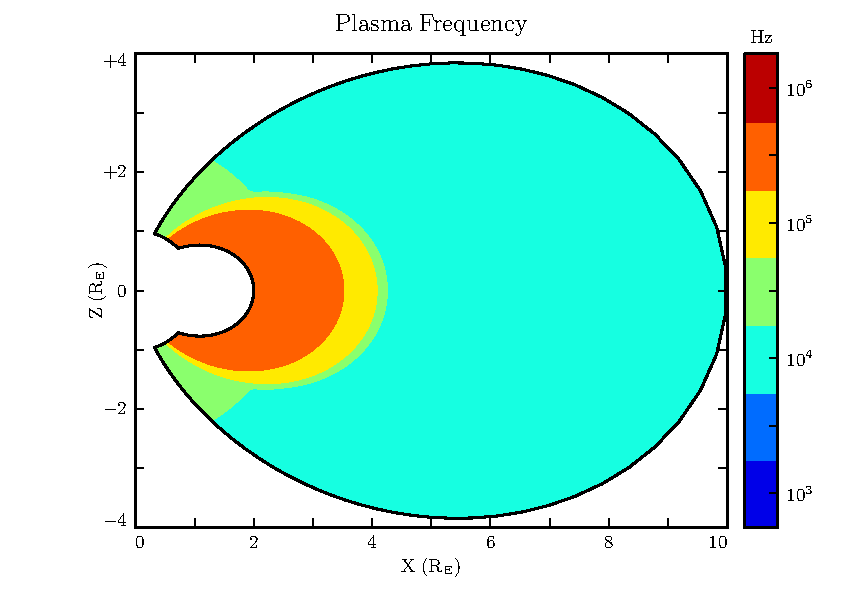
\includegraphics[width=\textwidth]{figures/op.pdf}
    \caption[Plasma Frequency Profile]{
      The plasma frequency reaches a peak value just under \SI{e7}{\radian/\second} near the equator. Outside the plasmasphere, its value is closer to \SI{e4}{\radian/\second}.  
    }
    \label{fig_op}
\end{figure}


%\todo{Generalized \ohmlaw, in case we decide we need it. Could talk through why all of the other terms are OK to neglect.  
%\begin{align}
%  \vec{E} + \cross{U}{B} & = 
%  \eta \vec{J} + \tfrac{\me}{n e^2} \lrb{
%    \tfrac{\partial}{\partial t} \vec{J} + \nabla \cdot \lr{ 
%      \vec{J} \, \vec{U} + \vec{U} \,\vec{J} +
%      \tfrac{1}{n e} \vec{J} \, \vec{J} } } +
%  \tfrac{1}{n e} \cross{J}{B} -
%  \tfrac{1}{n e} \div{ \vec{P_e} }
%\end{align}
%}

% =============================================================================
% =============================================================================
% =============================================================================
\section{Quantifying the Results}

\todo{How much does electron inertia matter? }

\todo{Note, again, that only the figures in the present chapter include electron inertia. Those in \cref{ch_azm,ch_rbsp} do not, for the sake of stability and computational cost. }

\todo{Integrate up a parallel electric field to see the potential difference. Compare to the relation seen by \cite{olsson_1996}, $J_\parallel \sim \Psi_\parallel$ by a proportionality constant of \SIrange{e-8}{e-10}{\S/\meter\squared}. }

\todo{Parallel electric fields, supposedly, only appear at high altitude. \cite{marklund_1997,carlson_1998}. }

% -----------------------------------------------------------------------------
% -----------------------------------------------------------------------------
% -----------------------------------------------------------------------------
\subsection{Parallel Electric Fields}
  \label{sec_inertia_fields}

\todo{Even side-by-side, the magnetic fields in an otherwise-identical run are not visibly affected by the addition of electron inertial effects. }

%\begin{figure}[H]
%    \centering
%    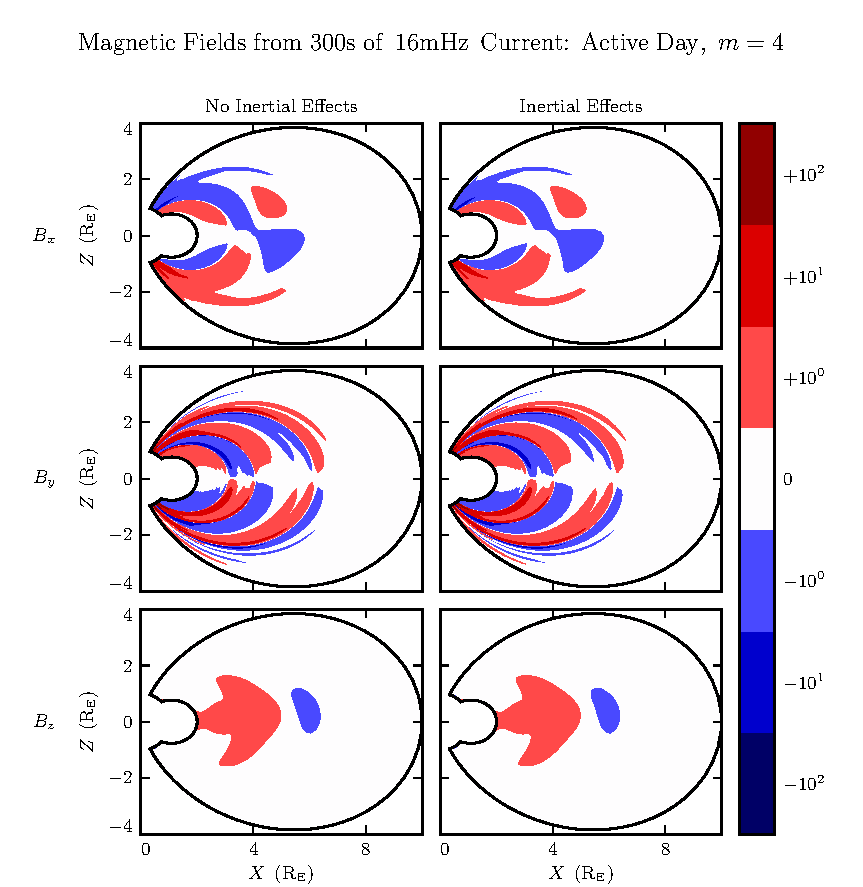
\includegraphics[width=\textwidth]{figures/B_1_004_016mHz.pdf}
%    \caption[Magnetic Fields With and Without Electron Inertia]{
%      The addition of electron inertial effects, with no other changes to the model, does not visible change the output. In a way, this is reassuring, since the alternative is to cast doubt on past work. 
%    }
%    \label{fig_B_1_004_016mHz}
%\end{figure}

\todo{The parallel electric fields do a bit better... after all, any change is a big change compared to zero. But they're still very small. }

With a bit of algebra, the meridional components of the dispersion tensor from \cref{sec_high_alt} provide a comparison of the parallel and perpendicular electric field magnitudes.
\begin{align}
  \frac{E_\parallel}{E_\bot} &= \frac{- k_\parallel k_\bot c^2 }{ \omega^2 - k_\bot^2 c^2 - \op^2 } \sim \frac{k^2 c^2 }{\op^2}
\end{align}

The electron inertial length $\frac{c}{\op}$ is on the order of \SI{1}{\km}, smaller than the wavelength of a field line resonance by three or four orders of magnitude. That is, at high altitude, the parallel electric field is expected to be smaller than the perpendicular electric field by a factor of \num{e7} -- perhaps more, depending on how closely the wave vector is aligned to the magnetic field. That seems fine -- note that \cref{fig_E_2_016_010mHz} shows that max $E_\parallel$ is 4 to 5 orders larger than max $E_\bot$... plus high altitude is the parallel field's minimum and the perpendicular field's maximum. 

\begin{figure}[H]
    \centering
    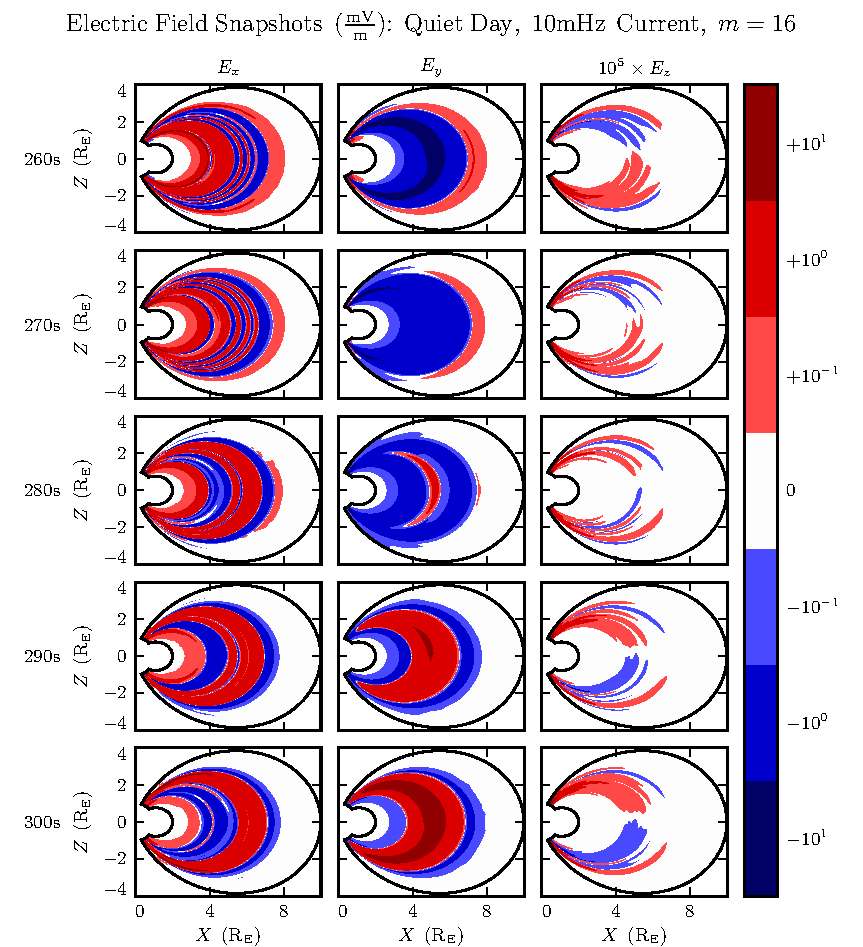
\includegraphics[width=\textwidth]{figures/E_2_016_010mHz.pdf}
    \caption[Parallel Electric Field Snapshots]{
      Parallel electric fields are smaller than perpendicular electric fields by at least four orders of magnitude.
    }
    \label{fig_E_2_016_010mHz}
\end{figure}

% -----------------------------------------------------------------------------
% -----------------------------------------------------------------------------
% -----------------------------------------------------------------------------
\subsection{Field-Aligned Current}
  \label{sec_fac}

\todo{The field-aligned current activity lines up with the Poynting flux. Poloidal Poynting flux is calculated from real $E_y$ and $B_x$. Toroidal Poynting flux is imaginary $E_x$ and $B_y$. The real component of the field-aligned current matches up with the poloidal, and the imaginary component lines up with the toroidal. }

\todo{Over the bulk of the simulation, each field is overwhelmingly either real or imaginary. However, that gets muddled at the ionosphere by the Hall conductivity (rather than being purely a function of azimuthal derivatives). }

\begin{figure}[H]
    \centering
    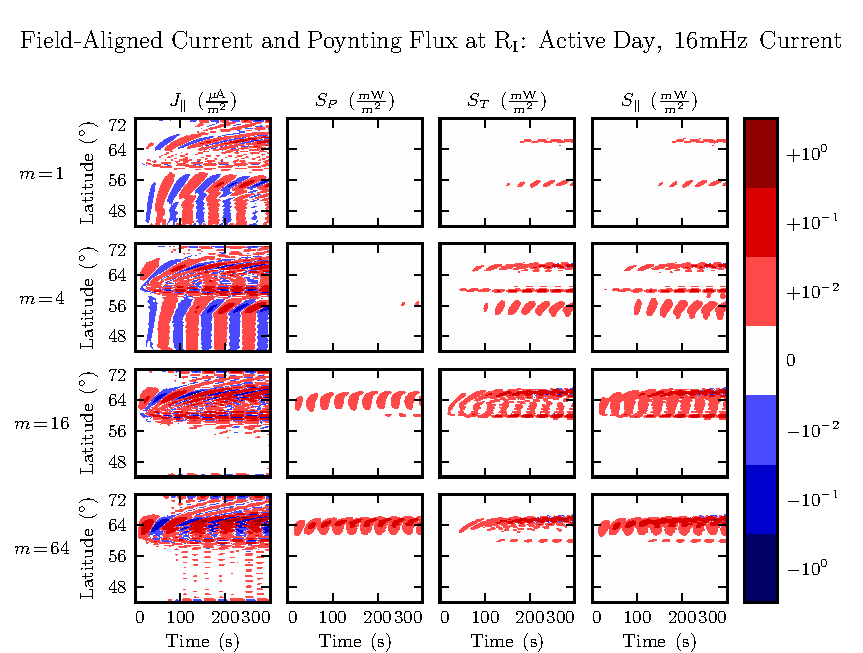
\includegraphics[width=\textwidth]{figures/JS_1_016mHz.pdf}
    \caption[Field-Aligned Current and Poynting Flux at the Ionosphere]{
      Perhaps unsurprisingly, field-aligned current structures at the ionospheric boundary line up with Poynting flux structures. The imaginary component of the current lines up with the toroidal Poynting flux (which is the product of imaginary $E_x$ and imaginary $B_y$), while the real current lines up with the poloidal Poynting flux ($E_y$ and $B_x$ are real). 
    }
    \label{fig_JS_1_016mHz}
\end{figure}

\todo{Notably, while the net Poynting flux is downward almost everywhere, field-aligned currents alternate between upward and downward flow. Perhaps this has to do with Poynting flux being a quadratic quantity while current is linear? }

The ``wigglies'' visible in the lower-left corner of \cref{fig_JS_1_016mHz} suggests overcorrection due to an improperly-coarse grid. See \cref{sec_lengths}. 

\todo{Field-aligned currents can be of significant size, but they're not particularly good at depositing energy in the ionosphere. As would be expected from energy conservation, $\nabla \cdot \vec{S}$ closely resembles $\vec{J} \cdot \vec{E}$, but only a vanishingly small portion of that is due to $J_z E_z$. }

\begin{figure}[H]
    \centering
    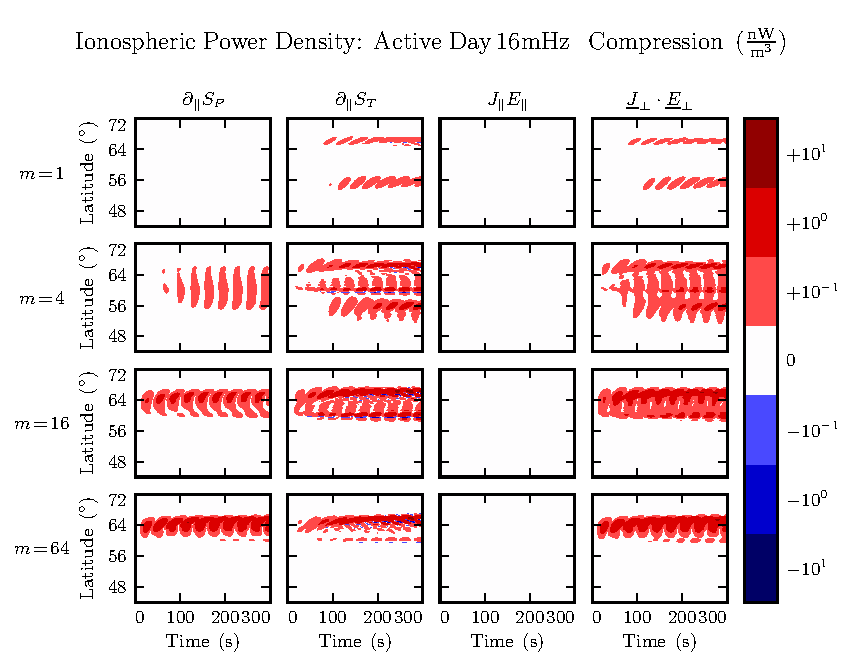
\includegraphics[width=\textwidth]{figures/JE_1_016mHz.pdf}
    \caption[Ionospheric Power Density]{
      While field-aligned currents can be of significant size, they are not particularly good at depositing energy in the ionosphere. Energy deposited by the Poynting flux matches closely with Joule dissipation from the perpendicular currents -- energy conservation! -- while $J_\parallel E_\parallel$ is smaller by several orders of magnitude. 
    }
    \label{fig_JE_1_016mHz}
\end{figure}

% -----------------------------------------------------------------------------
% -----------------------------------------------------------------------------
% -----------------------------------------------------------------------------
\subsection{Inertial Length Scales}
  \label{sec_lengths}

\todo{Are we really computing the electric fields faithfully? As touched on in \cref{sec_inertia_fields}, the perpendicular wavelength is important for determining the strength of the parallel electric field. This is because everything depends on derivatives, not magnitudes. }

\todo{A typical run has maximum perpendicular electric field on the order of \SI{10}{\mV/\meter}. Maybe a bit more. Field structures vary on the order of as little as $\sim\SI{1}{\degree}$. That could give up to $\curl{E} \sim \SI{e2}{nT/\second}$. In comparison parallel electric fields max out around \SI{e-3}{\mV/\meter}. If that varies as a scale of the inertial length -- as we expect, recalling \cref{sec_boris} -- that's order of \SI{1}{\km}, it could give $\curl{E} \sim \SI{1}{nT/\second}$. Plausibly large enough to have a visible effect. Note that the electron inertial length only needs to be resolved in the perpendicular direction, since that's where we're taking curls of the parallel electric field... which is the only quantity expected to change significantly (to lowest order) as a result of electron inertial effects. }

\todo{This poses a significant computational cost. Within the plasmasphere, the inertial length is on the order of \SI{0.1}{\km}. That's two-plus orders of magnitude smaller than the present grid. Moving the inner boundary from $L=2$ to $L=5$ makes up half of that. }

\todo{We do a few runs which sorta resolve the electron inertial length. It's about \SI{2}{\km}, and we get resolution down to \SI{0.7}{\km}. This is a factor of ten increase in resolution, and an additional factor of ten decrease in the time step (due to the drop in \Alfven crossing time). It's not enough. \cref{fig_Ez_inertial_length} is clearly not well-resolved. Those wigglies are probably about to cause a crash. }

\begin{figure}[H]
    \centering
    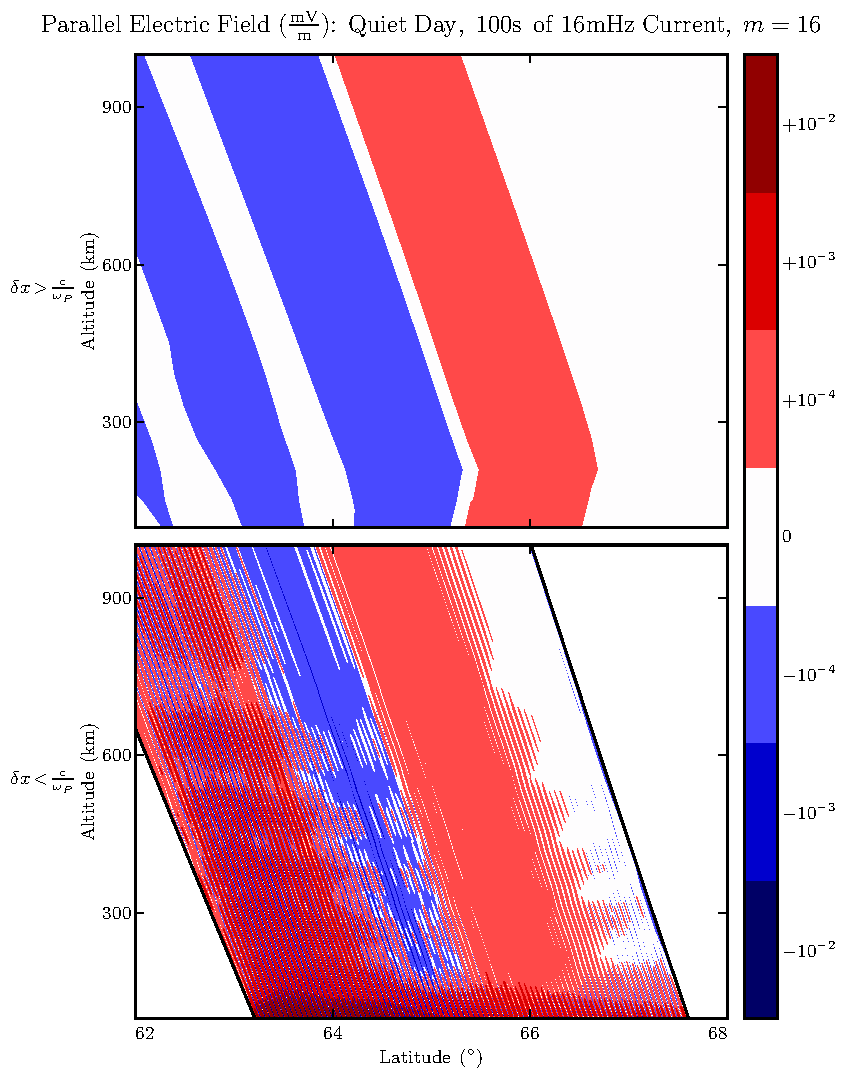
\includegraphics[width=\textwidth]{figures/Ez_inertial_length.pdf}
    \caption[Parallel Electric Fields by Perpendicular Grid Resolution]{
      The parallel electric field develops significant structure when the perpendicular grid resolution is smaller than the electron inertial length. Unfortunately, such runs are prohibitively expensive. The lower panel -- which still fails to resolve wave structure properly -- represents a 100-fold increase in computational time. 
    }
    \label{fig_Ez_inertial_length}
\end{figure}

\todo{The moral of the present section is that proper handling of electron inertial effects will probably show additional structure at small scales... but that simulating those structures is computationally expensive in terms of computational expense, even in 2.5D. }




